\chapter{Distributed Transactions}
A transaction becomes \textbf{distributed} if it invokes operations in \textit{several different servers.} These servers coordinate to \textbf{guarantee the same result}, and sometimes this operation is \textbf{not so easy} such that it will be necessary to \textbf{introduce a coordinator} entity or implement different coordination protocol.

We can identify two different type of transactions:
\begin{itemize}
    \item \textbf{Flat transactions:} are composed by a set of operations that are executed sequentially
    \item \textbf{Nested transactions:} are composed by subtransactions, which can run concurrently if they are at the same level
\end{itemize}

\begin{figure}[!h]
    \centering
    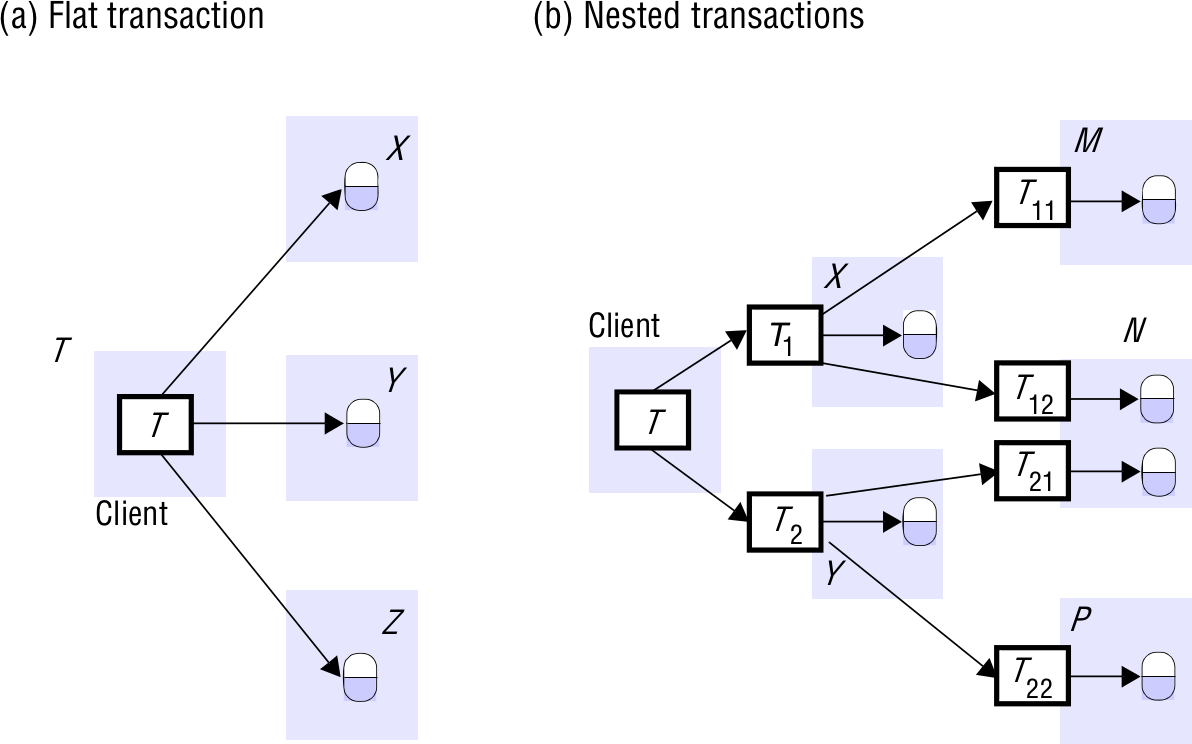
\includegraphics[width=.60\linewidth]{images/DistributedTransactions/distTransactions.png}
    \caption{Distributed transactions}
\end{figure}

\begin{itemize}
    \item In the flat transaction it invokes operations sequentially on objects in servers \(X\), \(Y\) and \(Z\)
    \item In the nested transaction, there are other two subtransactions \(T_1\) and \(T_2\) that open further transactions \(T_{11}\), \(T_{12}\), \(T_{21}\) and \(T_{22}\) which access objects at servers \(M\), \(N\) and \(P\). The subtransactions can run concurrently so, \(T_1\) and \(T_2\) are concurrent like \(T_{11}\), \(T_{12}\), \(T_{21}\) and \(T_{22}\).
\end{itemize}

\subsection{Coordinator of a distributed transaction}
Servers that execute requests as part of a distributed transaction need to be able to communicate with one another to coordinate their actions when the transaction commits.

A client \textit{starts a transaction} by sending an \textbf{openTransaction} request to a \textbf{coordinator}. It returns the resulting \textbf{transaction identifier} (TID), for example the pair (server ID, \# of local transaction). Coordinator at the end is responsible for committing or aborting it, moreover each server that manages an object used by a transaction is called \textbf{participant} in the transaction.
Each participant:
\begin{itemize}
    \item It executes operations of the transaction T
    \item It is responsible for keeping track of all of the recoverable objects involved in \(T\)
    \item It is responsible for cooperating with the coordinator to complete the \textit{commit} or call a \textbf{abortTransaction}
\end{itemize}

During the progress of the transaction, the coordinator records a list of references to the participants, and each participant records a reference to the coordinator.

\section{Atomicity}
When a distributed transaction comes to an end, the \textbf{atomicity} property of transactions requires that either \textit{all of the servers} involved \textbf{commit} the transaction or \textit{all of them} \textbf{abort} the transaction. To achieve this, one of the servers takes on a \textbf{coordinator role}.

There are essentially two protocols that try to guarantee atomicity among all the servers:
\begin{itemize}
    \item \textbf{One phase commit}
    \begin{itemize}
        \item The coordinator informs all the participants of the result
        \item It repeats the operation up to completion
        \item But in this way it can happen that \textbf{atomicity is not satisfied}
        \item If the client executes \textbf{commit} it does not allow a \textit{server to abort} if it is necessary, or it does not allow a \textbf{coordinator} to detect possible \textit{server faults}.
    \end{itemize}
    \item \textbf{Two phase commit}, is the most common and used algorithm, here all the participants can do abort. It is composed by two distinct phase:
    \begin{enumerate}
        \item \textbf{Voting phase:} 
        \begin{itemize}
            \item The \textbf{coordinator} sends a \textbf{canCommit?} request to each of the participants in the transaction
            \item When a \textbf{participant} receives a \textbf{canCommit?} requests it replyes with \textbf{Yes} or \textbf{No}
            \item Before voting \textit{Yes} it prepares to commit by saving objects in permanent storage.
            \item Otherwise it responds \textit{No}, the participant aborts
        \end{itemize}
        \item \textbf{Decision phase:}
        \begin{itemize}
            \item The \textit{coordinator collects the votes}, if there are \textit{no failures} and all the votes are \textbf{Yes} the coordinator decides to \textbf{commit} the transaction and sends a \textbf{doCommit} request to each of the \textit{participants}.
            \item Otherwise the \textit{coordinator decides} to \textbf{abort} the transaction and send \textbf{doAbort} requests to all \textit{participants} that voted \textbf{Yes}
            \item \textit{Participants} that voted \textbf{Yes} are waiting for a \textbf{doCommit} or \textbf{doAbort} request from the coordinator. When a participant receives one of these messages it acts accordingly and in the \textit{case of} \textbf{commit}, makes a \textbf{haveCommitted} call as confirmation to the coordinator.
        \end{itemize}
    \end{enumerate}
\end{itemize}

\begin{figure}[!h]
    \centering
    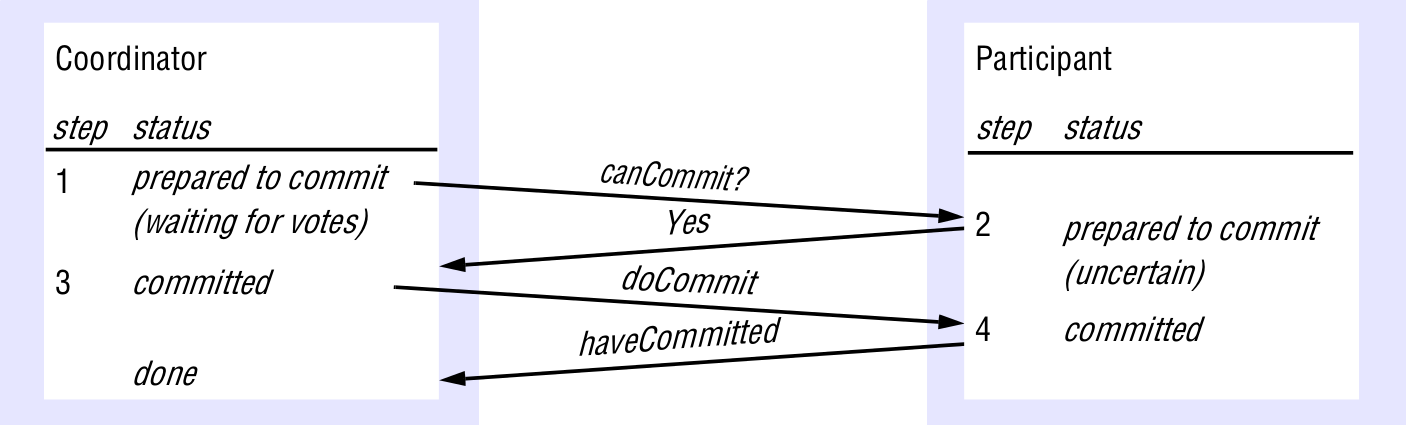
\includegraphics[width=.80\linewidth]{images/DistributedTransactions/twoPhaseCommunication.png}
    \caption{Communication in two phase commit protocol}
\end{figure}

\section{Fault and performance management}
There are various stages in the protocol at which the coordinator or a participant \textbf{cannot progress} until it receives another request or reply from one of the others.

In order to avoid that some entities wait for a long time without any probability to get an answer it is introduced the usage of \textbf{timeouts}. For example if a participant that is waiting for a \textbf{doCommit} message set a timeout, if the \textit{timeout fires} it will \textbf{abort} the transaction.

The critic point for fault management happens if the \textbf{coordinator crashes} after that it sent \textbf{doCommit} to all the partecipants. The problem consists on the fact that \textbf{later it will be no able to check if all the participants have commited or not.}


\section{Two phase commit protocol for nested transactions}
As we have seen before nested transactions are composed by top-level transaction and subtransactions. When a subtransaction completes, it makes an independent decision either to commit provisionally or to abort.

A \textbf{provisional commit} is different from being preared to commit: \textit{nothing is backed up in permanent storage.}

After all subtransactions have completed, the provisionally committed ones participate in a two-phase commit protocol. In other words provisional commit means that coordinator and transactional servers are ready to commit subtransaction but they have not yet done so.

\begin{figure}[!h]
    \centering
    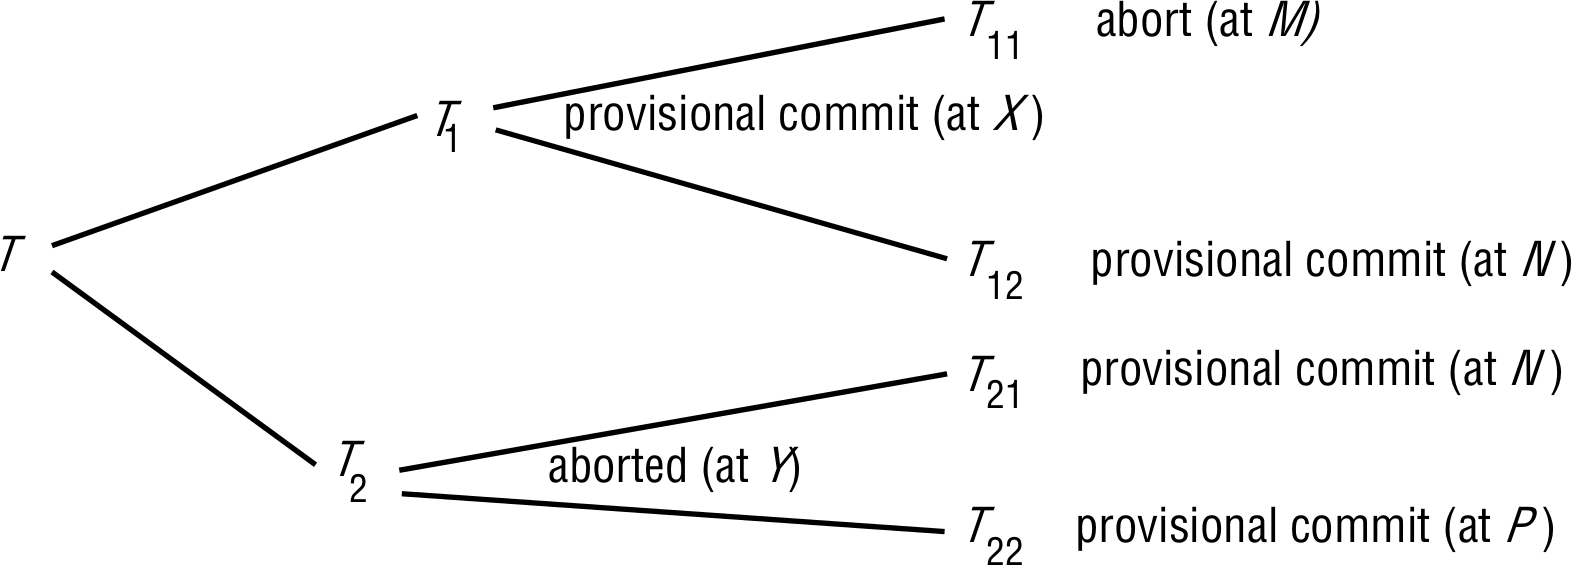
\includegraphics[width=.60\linewidth]{images/DistributedTransactions/DistnestedTransactions.png}
    \caption{Distributed nested transaction}
\end{figure}

From the previous picture we can see that even if \(T_{11}\) abort \(T_1\) in this example is in provisional commit state. It can happen if the transaction \(T_{11}\) is not considered fundamental: example multiple thread to find an element, if at least one of this thread find the element I can ignore the other ones. But there are also case in which \(T_{11}\) plays a fundamental role, and in this case \(T_1\) should abort.


\section{Protocol realization}
\textbf{Two phase commit protocol} can be realized as:
\begin{itemize}
    \item \textbf{Flat:} the coordinator of the top-level transaction sends  \textbf{canCommit?} messages to the coordinators of all the previous transactions in the \textbf{provisional commit list}. Partecipants that receive the message replies with it vote Yes or No if they can commit or not.
    \item \textbf{Hierarchical:} the coordinator of the top-level transaction communicates with the coordinators of the subtransactions for which it is the immediate parent. It sends \textbf{canCommit?} messages to each of them, which in turn pass them on to the coordinators of their child transactions.
\end{itemize}


\section{Concurrency control for distributed transactions}
The servers apply to their own objects the protocols of concurrency control for distributed transactions like \textbf{locking}, \textbf{optimistic} and \textbf{timestamp}. Servers must coordinate to ensure serial equivalence.

\subsection{Locking}
\begin{itemize}
    \item In a distributed transaction, the locks on an object are held locally
    \item The \textbf{local lock manager} can decide whether to grant a lock or to make the requesting transaction wait.
    \item When locking is used for concurrency control, the objects remain locked and they are unavailable for other transactions during the atomic commit protocol. Since each server manages the locks locally and independently from the others, it is possible that different servers may impose different orderings on transactions. These different orderings can lead to cyclic dependencies between transactions, giving rise to a distributed deadlock situation.
    
    \begin{figure}[!h]
    \centering
    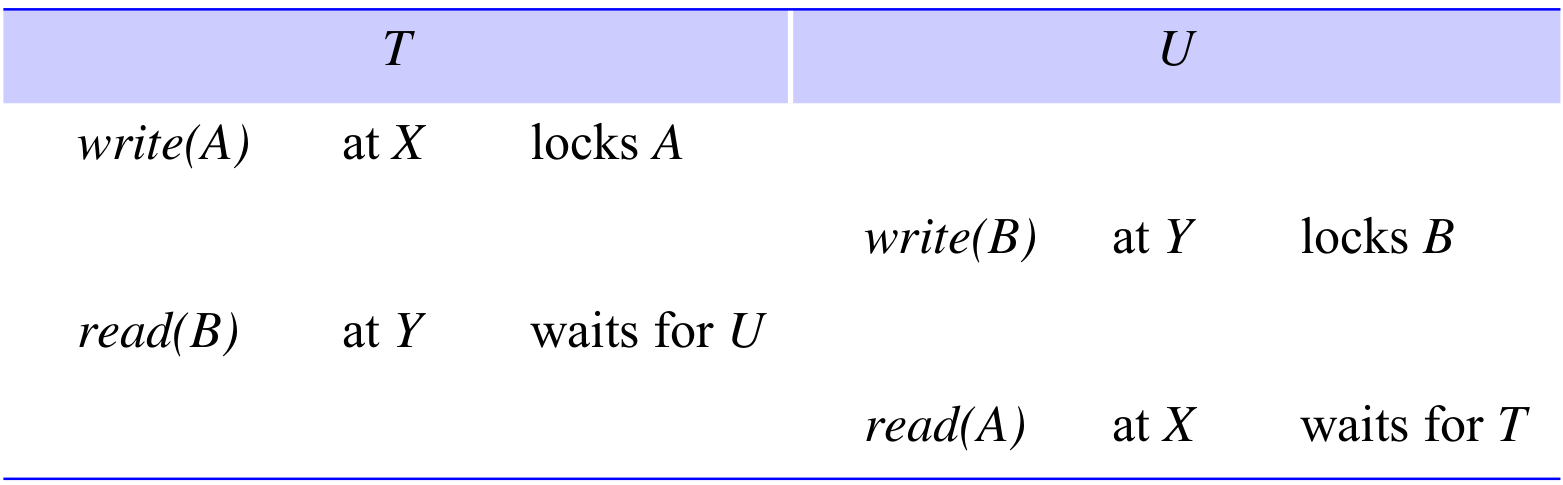
\includegraphics[width=.60\linewidth]{images/DistributedTransactions/locking.png}
    \caption{Locking in distributed transactions}
    \end{figure}
    
\end{itemize}

\subsection{Timestamp}
In distributed transactions, we require that each coordinator provides \textbf{globally unique timestamps}.
\begin{itemize}
    \item It is provided to the client by the coordinator the first time
    \item The transaction timestamp is passed to the coordinator at each server whose objects perform an operation in the transaction
    \item To achieve the same ordering at all the servers, the coordinators must agree as to the ordering of their timestamps
\end{itemize}

\subsection{Optimistic}
With optimistic \textit{concurrency control}, each transaction is \textbf{validated before commit execution}.
\begin{itemize}
    \item  Transaction numbers are assigned at the beginning of the validation phase and transactions are serialized according to the order of their transaction numbers
    \item A distributed transaction is validated by a collection of independent servers
\end{itemize}

\section{Distributed deadlock}
Most deadlock detection schemes operate by \textbf{finding cycles} in the transaction \textit{wait-for graph}. In a distributed system involving \textbf{multiple servers} being accessed by multiple transactions a global \textit{wait-for graph} can be constructed by the local ones.

There can be a cycle in the global wait-for graph that \textit{is not in any single local one}, there can be in fact a \textbf{distributed deadlock}.

We can understand so that, to detect a \textbf{distributed deadlock}, it is required to find a \textbf{cycle in the global transaction} \textit{wait-for graph} that is distributed among the servers that were involved in the transactions.
\newpage
\begin{figure}[!h]
    \centering
    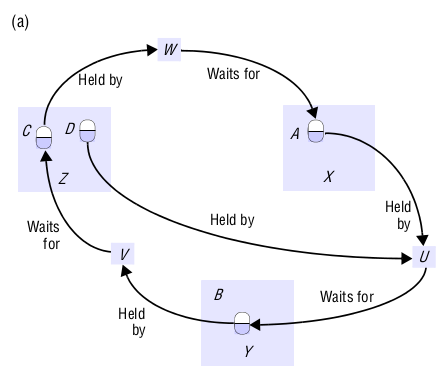
\includegraphics[width=.60\linewidth]{images/DistributedTransactions/distributedDeadlock.png}
    \caption{Example of global \textit{wait-for graph}}
\end{figure}

We have three strategy to ensure distributed deadlock:
\begin{itemize}
    \item \textbf{Centralized deadlock detection:} in which one server takes on the role of \textbf{global deadlock detector}. When it finds a circle it decide what to do and what transaction to abort. This method is not a good idea since it \textbf{depends on the server} to carry it out.
    \item \textbf{Phantom deadlock:} which is a deadlock that is "detected" but it is not really a deadlock. In other word there is a chance that one of the transactions that holds a lock will meanwhile have released it, in which case the deadlock will no longer exist.
    \item \textbf{Edge chasing:} in which the \textit{global wait-for graph} \textbf{is not constructed}, but each of the servers involved has \textbf{knowledge about some of its edges}. The servers attempt to \textit{find cycles} by forwarding messages called \textbf{probes}. When a cycle is detected, a transaction in the cycle is aborted to break the deadlock.
\end{itemize}

\section{Transaction recovery}
This propriety tell us that all the effects of committed transactions and non of the aborted one are reflected in the object they refer. This definition could be expanded by other two aspects:
\begin{itemize}
    \item \textbf{Durability:} requires that objects are saved in permanent storage and will be available indefinitely thereafter
    \item \textbf{Failure atomicity:} requires that effects of transactions are atomic even when the server crashes.
\end{itemize}
We will assume that when a server is running it keeps all of \textit{its objects} in its \textbf{volatile memory} and records \textit{its committed objects} in a \textbf{recovery file}.

This two propriety can be merged into a single mechanism called \textbf{recovery manager}. Its \textbf{tasks} are:
\begin{itemize}
    \item Save objects in permanent storage for committed transactions.
    \item Restore the server’s objects after a crash
    \item Reorganize the recovery file to improve the performance
    \item Manage recovery file
\end{itemize}

Any server that provides transactions needs to keep track of the objects accessed by client's transactions. At each server, an \textbf{intentions list} is recorded for all of its currently active transactions.
\begin{itemize}
    \item An intentions list of a particular transaction contains a \textbf{list of the references} and the \textbf{values} of all the \textit{objects that are modified} by that transaction.
    \item When a transaction is \textbf{committed}, that transaction’s \textit{intentions list} is used to \textbf{identify the objects it affected}.
    \item Each object in the \textit{recovery file} is associated with a particular transaction by \textbf{saving the intentions} list in the \textit{recovery file}.
\end{itemize}
Two approaches can be used to create a \textit{recovery file}: \textbf{logging} and \textbf{shadow version}.

\subsection{Logging}
In the logging technique, the \textit{recovery file} represents a log containing the \textbf{history} of all the transactions performed by a server. This \textit{history} contains values of objects, transaction status entries and transaction intentions lists.

During the normal operation of a server, its recovery manager is called whenever a transaction prepares to commit, commits or aborts a transaction. When the server is \textbf{prepared to commit a transaction}, the recovery manager appends
\begin{itemize}
    \item All the objects in its intentions list to the recovery file
    \item Followed by the current status of that transaction together with its intentions list
\end{itemize}


\section{Shadow versions}
The \textbf{shadow versions} technique is an alternative way to \textit{organize a recovery file}. It uses a \textbf{map} to \textit{locate versions of the server’s objects} in a file called a \textbf{version store}. The map associates the identifiers of the server’s objects with the positions of their current versions in the version store.

When a transaction is prepared to commit, any of the objects changed by the transaction are appended to the version store, leaving the corresponding committed versions unchanged.

To restore the objects when a server is replaced after a crash, its recovery manager reads the map and uses the information in the map to locate the objects in the version store.

\subsection{Recovery of the two-phase commit protocol}
The recovery management described previously, must be \textbf{extended} to deal with any \textit{transactions} that are performing the \textbf{two-phase commit protocol} at the time when a server fails. Thus the recovery managers use two new status value for this purpose: \textbf{done} and \textbf{uncertain}.

\begin{itemize}
    \item A \textbf{coordinator} uses \textbf{committed} to indicate that the outcome of the vote is \textbf{Yes} and \textbf{done} to indicate that the \textit{two-phase commit protocol} is complete.
    \item A \textbf{participant} uses \textbf{uncertain} to indicate that it has voted \textbf{Yes} but does not yet know the outcome of the vote.
\end{itemize}
So the \textbf{two phases} are:
\begin{itemize}
    \item \textbf{First phase}, when the \textit{coordinator} is prepared to \textbf{commit}, its recovery manager adds a coordinator entry to its recovery file.
    \begin{itemize}
        \item \textbf{It votes Yes:} its recovery manager records a \textit{participant entry} and adds an \textbf{uncertain transaction} status to its recovery file as a \textit{forced write}.
        \item \textbf{It votes No:} it adds an \textbf{abort transaction} status to its recovery file.
    \end{itemize}
    \item \textbf{Second phase:} the recovery manager of the coordinator adds either a \textit{committed} or an \textit{aborted} transaction status to its recovery file, according to the decision
\end{itemize}
